%
%
% A (non-exhaustive) list of TODOs:
% - expand the calculating holevo section
% - find somewhere for my nice line about the quantum protocol being ``agnostic'' to the classical steps
% - talk about how interpretation of \chi differs between qdsb and qdsf
% Q: do I want more chat about the large figure?
% - make new figure about the roles (just gonna use stefan's figure for now)
% - make sure I show how each protocol can be made more ``experimentally realistic''.
% - ensure that my description of QDSb is identical in style to QDSf from earlier
% - add appendix where I put the states for QDSb under each attack.
%



\chapter{Agile quantum cryptography}\label{chapter:aqc}
Goal of chapter: introduce and make explicit the concept of quantum agility in quantum cryptography. Join together several threads from the previous two chapters. This chapter can be viewed as a "bonus" to the QDS and QSS chapters.

\iffalse
Key things I want to present, in roughly the order that I want to present them:

\begin{itemize}
\item Discussion of agility and why it might be desirable. Motivate it in terms of my two literature reviews.
\item Modification of QDS protocol from earlier to be agile with QSS (i.e. introduce protocol QSS-b and prove its security (inc postselection)). Have some graphs of its behaviour
\item Bring in QKD from the literature (Papanastasiou2018). Have some graphs of its behaviour and discussion of how it relates to my thesis.
\item Talk about the experiment (emphasise that it is not my work). I can have some plots of raw data (opendata), and make graphs of data points which I received.
\item Analysis of the data under each protocol with discussion of how results from previous chapters are modified to make them more realistic
\item Graphs of performance at different data parameters
\item Table from the AQC paper $\leftarrow$ this can be the climax of this section
\item star graph of QDS
\item Discussion of how our analysis motivates agility
\item Outlook/next steps
\end{itemize}
\fi

\section{Introduction}

% Review some things from my previous two literature reviews
We have observed over the past two chapters, and in our overviews of quantum cryptography in Chapter~\ref{chapter:crypto_intro}, that several quantum cryptographic protocols are intimately related. As Simmons noted as his abstract to Ref.~\cite{Simmons1990a},

\begin{center}\emph{``Secret sharing is simply a special form of key distribution''}\end{center}



\noindent and so we have seen close connections between QKD and QSS, and noted that QSS may be interpreted simply as QKD performed between one player (dealer) and several players (recipients of the secret). We have also remarked that the secret sharing task may be performed pseudo-classically, by first encrypting channels using QKD and then using an unconditionally secure classical secret sharing protocol, of which there are many \cite{Schneier1996}. It was noted in Refs.~\cite{Hillery1999, Chen2005a, Wu2016, Ottaviani2017b} that QSS is related to quantum conferencing, and often the same hardware setup may be used to perform both tasks. And in Ref.~\cite{Grice2019} it was explicitly demonstrated that a sequential round-robin QSS protocol can also be used to perform QKD between any two players. 

Moving to the QDS literature, ever since discovery of practical QDS requiring neither quantum memory, entanglement, nor an optical multiport it has been accepted that there are close links between QDS and QKD. Ref.~\cite{Wallden2015} explicitly builds their QDS protocol to use QKD hardware, while Ref.~\cite{Roberts2017} realise a setup which can, with minimal hardware modification, perform either QDS, or QKD with additional MDI capabilities. Refs.~\cite{Collins2016, Yin2017, Yin2017c, An2019, Roberts2017} remark that QDS differs from QKD only in the classical postprocessing, and Ref.~\cite{Wei2018} designs a QSS scheme using the same principles as differential-phase-shift based QKD \cite{Sasaki2014}. Indeed, many papers build their security proofs on techniques designed first for QKD \cite{Kogias2017, Grice2019, Wei2018, Grice2015, Armstrong2015}.

%We therefore might ask 

It should be clear that the field of quantum cryptography is far broader and more interesting than just QKD \cite{Broadbent2015}. As the field moves closer towards practical implementation of diverse quantum cryptographic protocols, one must consider not only the unconditional security of the underlying protocol but also its ease of implementation. As protocols are designed with minimal and often overlapping hardware requirements we may ask the following questions:
\\
\par
Q1:\emph{ given a particular hardware setup, which quantum protocols can I perform?}
\\
\\
\noindent Or, desiring a large-scale quantum cryptographic network:
\\
\par
Q2:\emph{ given a deployed network architecture, which quantum protocols can I perform with minimal disruption?}
\\
\\
\noindent Both of these questions will have deep impacts on the success of a future large-scale quantum network. \MT{Chat more about the networks. Mention DV over installed fibers results from recent years. (Did they require dedicated hardware?)}

We have already even seen several quantum routes to perform the same task. For example, by utilizing prior QKD between all players it is possible to perform digital signatures \cite{Wallden2015, Amiri2016a} or secret sharing \cite{Schneier1996} using unconditionally secure classical algorithms, and indeed this may often be preferable to protocols requiring large entangled states \cite{Gottesman2001, Hillery1999}. Alternatively, in a distributed quantum computing setup which can easily generate and distribute entanglement, protocols such as Refs.~\cite{Bell2014, Kogias2017} may be advantageous if they take advantage of already accessible hardware. The comparison between the many different routes to the same task is rarely straightforward and is often more involved than a simple key rate comparison. 

In addition to considering the performance of unconditionally secure protocols, the questions Q1 and Q2 push us to consider practical quantum cryptographic protocols which may perform well but not yet offer full unconditional security against an infinitely powerful eavesdropper. This may particularly be the case as new side-channel attacks are designed and discovered in existing quantum cryptographic protocols. Indeed, throughout the history of \emph{classical} cryptography, development of new cryptoystems have often occurred in response to the breaking of a system which was previously believed secure. Perhaps cynically, one could even view crpytographic history has a "cat-and-mouse" race between cryptographers and cryptanalysists.%: cryptographers trying to develop new protocols and harden their security; cryptanalysts endeavouring to secretly break them and intercept their messages. 

The replacement of a newly-insecure cryptosystem is difficult, expensive and time-consuming. In response to this problem in classical cryptography there has recently been a push towards so-called \emph{crypographic aglity} (crypto-agility) \cite{Sullivan2009, Chen2016} with a key motivator being the development of quantum computers. %\MT{I want to mention somewhere the google chrome trial.} 

\subsection{(Quantum) crypto-agility}

One of the main ideas of crypto-agility is the existence of a middleware which interacts both with the software application layer (user) and the underlying cypto-core (algorithm). This is accomplished in Ref.~\cite{Sullivan2009} for example by ensuring that written code is kept as abstract as possible without hard-coding the secure protocols which are used by the code. This allows for flexible switching between underlying algorithms and keeps the top-level code agnostic as to which secure algorithms are being used. When the security of the underlying algorithm is weakened it becomes easy to simply replace the algorithm with a new or modified one, without changes to the rest of the computational architecture. Failures to allow a system to respond to new cryptographic threats like this can be at best embarrassing, and at worst costly or life-threatening \cite{Schneier2016, Schneier2017}. The key idea of crypto-agility is depicted in Fig.~\ref{fig:agility}a. 


\begin{figure}[htp]
\centering
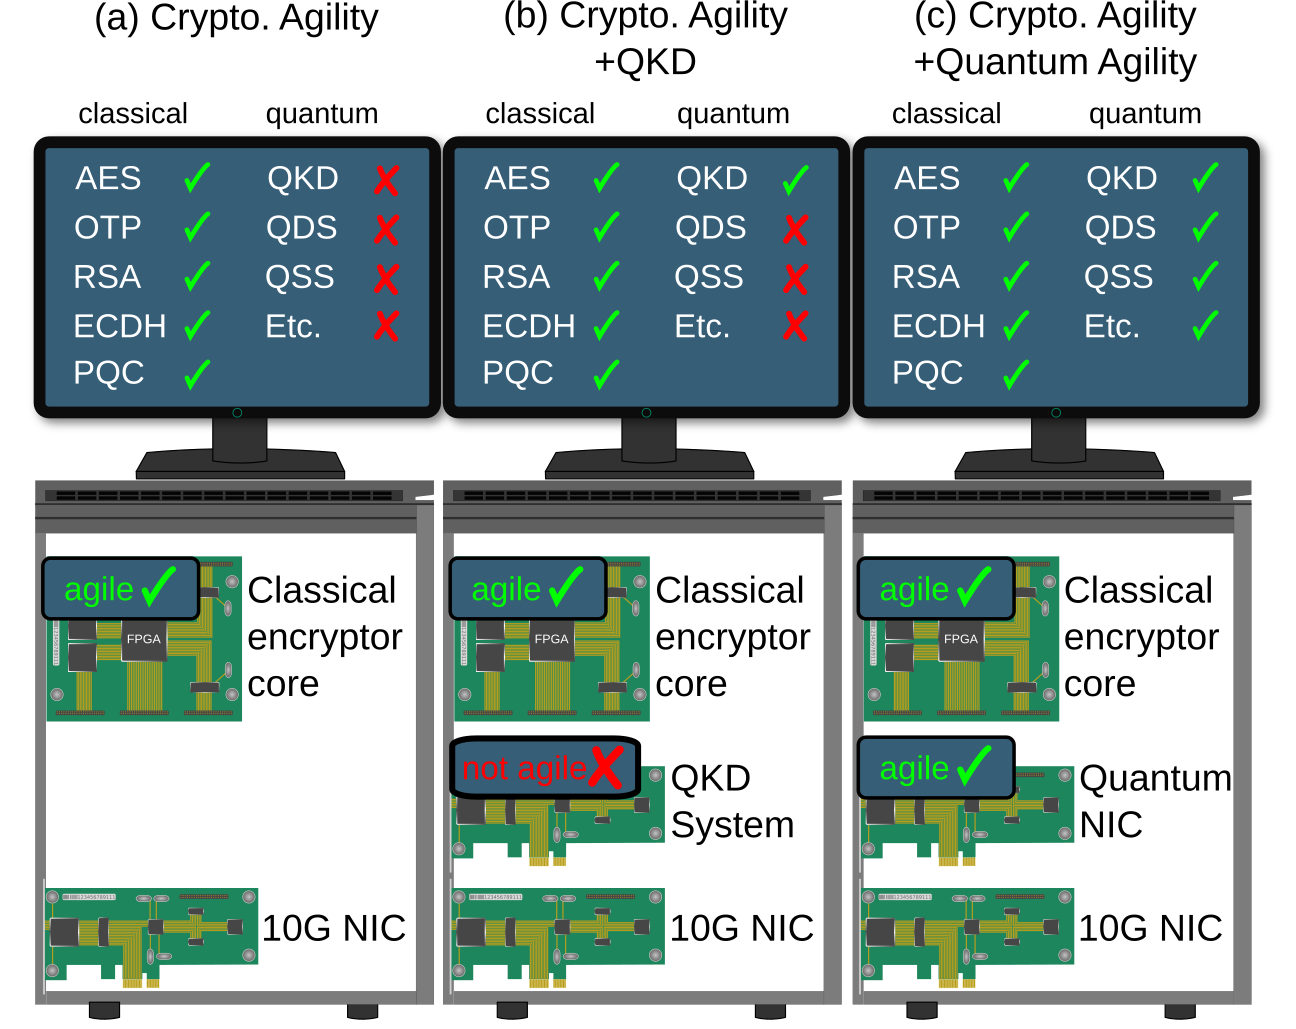
\includegraphics[draft=false]{aqc/Fig1-qagility}
\caption{\label{fig:agility} An agile cryptographic system involves a middleware which interacts between the user and the underlying crypto-core. The crypto-core (algorithm) may be readily replaced without affecting the rest of the software architecture. (a) Currently implemented classical crypto-agility. (b) QKD-assisted crypto-agility, in which several classical protocols may be run over secure channels first encrypted via a QKD link. (c) Full quantum crypto-agility which can choose interchangably between many different quantum protocols. Classical algorithms and quantum algorithms can be replaced as necessary. The classical protocols displayed are: Advanced Encryption Standard (AES), One-time Pad (OTP), Rivest-Shamir-Adleman (RSA), Elliptic-Curve Diffie-Hellman (ECDH) and post-quantum cryptography (PQC). \emph{Picture credit: Stefan Richter in Ref.~\cite{Richter2020}}}
\end{figure}


The framework of classical crypto-agility seems ideal to help us answer Q1 and Q2. It is natural to separate the application layer (the task to be performed) from the underlying algorithm (which we may call a "quantum crypto-core"), in order to envisage a future quantum-software library which can select between the appropriate underlying algorithm based on the desired task and the available network hardware. We are then motivated to explore the quantum analogue of classical crypto-agility as a step towards efficient and flexible quantum communications networks.

%\MT{Now, talk about different views of quantum agility, with reference to Fig.1}
%\MT{I think I should only talk about CV+heterodyning and compatibility with infrastructure when I come to talk about the protocols, since it is in a sense a particular instance of the problems I am discussing in this section.}

%The following view of quantum crypto-agility (or quantum agility) can be thought of as analogous to a framework for quantum computing in which (this sentence doesn't really add much)

%\MT{-------------------}


There are two potential ways to translate the idea of classical crypto-agility into the quantum realm. We depict them both in Figs.~\ref{fig:agility}b,~\ref{fig:agility}c. The first we refer to as ``QKD-assisted crypto agility'', which may be seen as a generalization of qCSS, Sec.~\ref{sec:qss_qcss} and the classical signatures protocols \cite{Wallden2015, Amiri2016a} which implicitly require QKD first in order to remain secure. The QKD system delivers fresh secure random keys which may be used for many different protocols. This is the stance taken by the ETSI QKD ISG $004$ \cite{ETSI004} and $014$ \cite{ETSI014} standardization efforts which specify interface design between a QKD system (hardware) and the key management system (software). We expect that this QKD-assisted crypto agility will form an important cornerstone for future quantum networks. %This viewpoint on agility is displayed in Fig.~\ref{fig:agility}~(b).

However, as was shown in Ref.~\cite{Amiri2016} in the context of QDS, it is not always optimal to perform QKD and then a classical protocol, since there may be channels over which QKD is not possible, or hardware setups over which the costly reconciliation procedures are difficult. The second viewpoint of quantum crypto-agility may thus be referred to as a ``fully quantum crypto agility'', Fig.~\ref{fig:agility}c. Rather than building upon an underlying and fixed QKD system, such a setup should have the capability to perform multiple quantum communication protocols. This should use the so-called \emph{quantum network interface card} in Fig.~\ref{fig:agility}. This viewpoint recognises the fact that multiple quantum cryptographic protocols differ only in classical postprocessing but share quantum stages and so a full QKD protocol may not be required. %In this case the choice of quantum protocol to perform is reduced simply to an update 
In a deployed system the ability to perform new quantum cryptographic protocols may then be reduced to a mere upgrade of classical firmware.


%\MT{Do I want a statement along the lines of "It is important to relaize that the transfer of the crypto-agility idea to the field of quantum cryptography changes its meaning..." from the paper?}

In Fig.~\ref{fig:big_agile} we present an example of an agile quantum communications stack which expresses the viewpoint of Fig.~\ref{fig:agility}c. The stack provides clear separation between the user (software layer) and the physical hardware layer, and may be interpreted as analogous to recent work on compilers for quantum computers \cite{Killoran2018, qiskit, Murali2019}.

%\MT{chat about this picture.}
\begin{figure}[htp]
\floatbox[{\capbeside\thisfloatsetup{capbesideposition={left,top},capbesidewidth=4cm}}]{figure}[\FBwidth]
{\caption{\label{fig:big_agile} Agile quantum communications stack following the viewpoint of Fig.~\ref{fig:agility}c. The \emph{user app} layer allows a user to select a task they wish to perform, (e.g. message encryption, message authentication, secret sharing). The agile middleware provides a separation between the user (software) and underlying quantum crypto-system (hardware). The \emph{primitive} layer selects the desired cryptographic primitive (e.g. QKD, QDS, QSS, RSA), and instructs the \emph{protocol and hardware abstraction} layer to run the protocol via a library of known functions (e.g. ``send coherent state'', ``perform heterodyne detection''). These commands are interpreted by the \emph{hardware} layer and sent to the physical hardware setup. The agile system should be flexible and allow for switching between different tasks, different protocols and different hardware setups. \emph{Picture credit: Stefan Richter in Ref.~\cite{Richter2020}}}}
{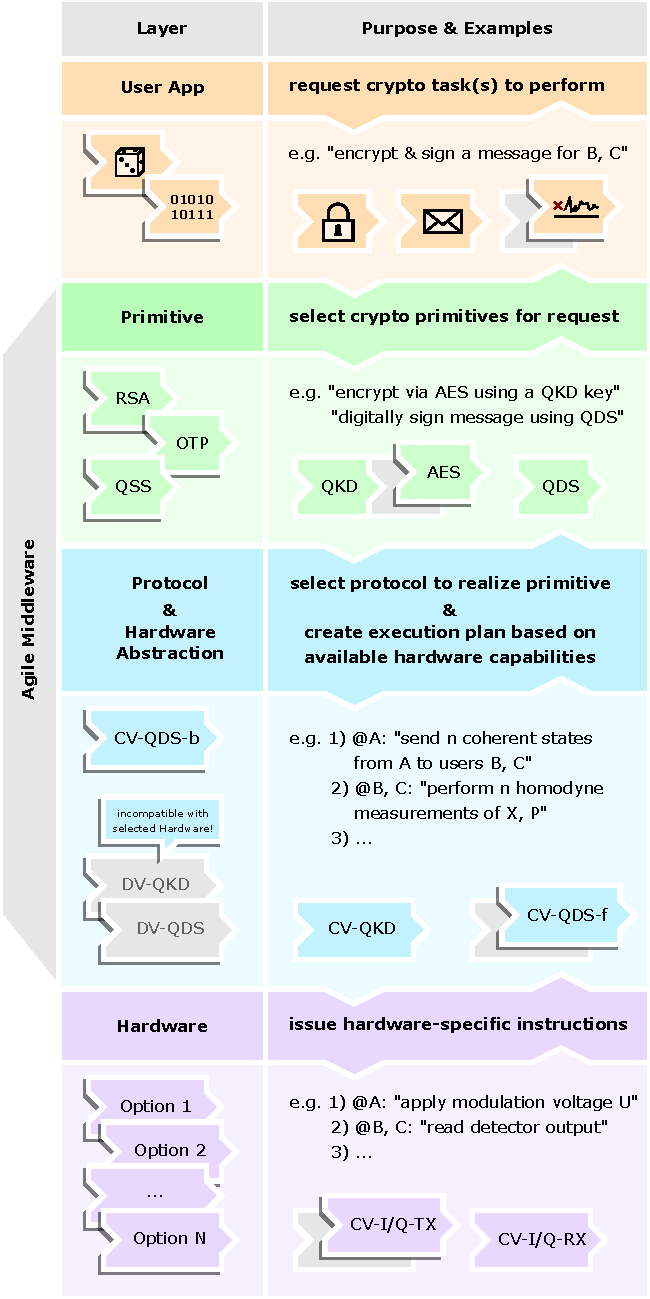
\includegraphics[draft=false, width=10cm]{aqc/layers_5}}
\end{figure}


\iffalse
\begin{figure}[htp]
\centering
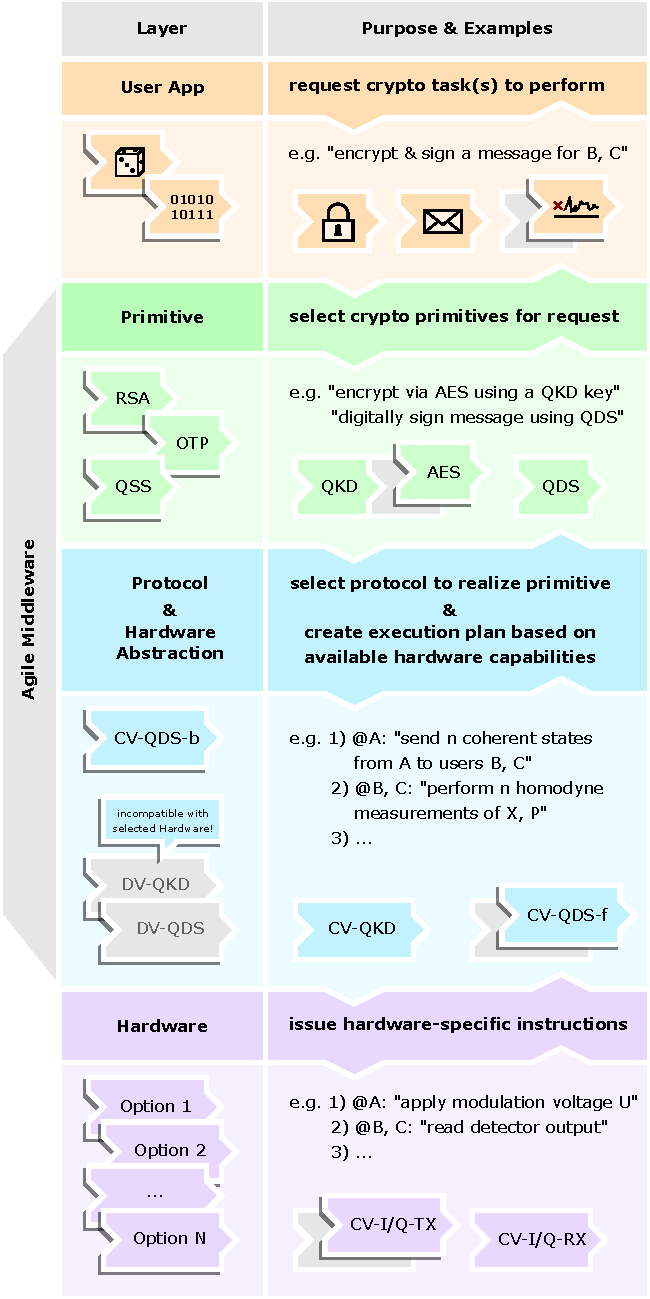
\includegraphics[draft=false]{aqc/layers_5}
\caption{\label{fig:big_agile} Agile quantum communications stack following the viewpoint of Fig.~\ref{fig:agility}c. The \emph{user app} layer allows a user to select a task they wish to perform, (e.g. message encryption, message authentication, secret sharing). The agile middleware provides a separation between the user (software) and underlying quantum crypto-system (hardware). The \emph{primitive} layer selects the desired cryptographic primitive (e.g. QKD, QDS, QSS, RSA), and instructs the \emph{protocol and hardware abstraction} layer to run the protocol via a library of known functions (e.g. ``send coherent state'', ``perform heterodyne detection''). These commands are interpreted by the \emph{hardware} layer and sent to the physical hardware setup. The agile system should be flexible and allow for switching between different tasks, different protocols and different hardware setups. \emph{Picture credit: Stefan Richter in Ref.~\cite{Richter2020}}}
\end{figure}
\fi

\clearpage
\section{CV agile quantum systems}
%Make sure to acknowledge that this text is very similar to Richter2020 Section 3. Which is fine, since I wrote it and it wasn't edited by coauthors. 

To illustrate the above discussion, in this section we will introduce and analyse two quantum systems capable of implementing multiple protocols over the same hardware setups. The protocols differ only at the level of classical postprocessing. Our hardware setup is explicitly designed with question Q$2$ in mind, and with a desire for compatibility with currently deployed network architecture. The systems therefore are fully continuous-variable, and relying on distribution of phase-modulated QPSK coherent states and their heterodyne phase detection \cite{Agrawal2008} rendering each system highly compatible with deployed telecommunications infrastructure. This paves the way to an integration between our agile systems into deployed communication links which can run with up to $100$~GHz sending rate \cite{Khan2015, Khan2016}. In Sec.~\ref{sec:aqc_experiment} we describe and analyse an experimental implementation of the agile systems discussed here.

We will consider the following tasks:

\textbf{QDS - quantum digital signatures}: allows for secure authentication of a classical message. It has been explicitly demonstrated that because of its small overhead, QDS may run over channels for which QKD is insecure \cite{Amiri2016}.

\textbf{QSS - quantum secret sharing}: allows for secure distribution of a classical secret among a conspiracy of potentially dishonest recipients.

\textbf{QKD - quantum key distribution}: allows for secure key distribution of identical randomly-generated bits between players. These keys may them be used for encryption via one-time pad\cite{Schneier1996}.

The tasks QDS and QSS are discussed in Chapters~\ref{chapter:qds},~\ref{chapter:qss} above, while the reader is referred to \cite{Laudenbach2017, Scarani2009} for review of QKD. The tasks QDS and QSS are inherently multipartite, while QKD is inherently bipartite\footnote{Though note the existence of its multipartite generalization - quantum conferencing \cite{Ottaviani2017b, Ottaviani2019}}. In what follows we will use quantum networks with three players to allow for multipartite tasks, while also allowing for bipartite QKD to be performed.

\begin{figure}[htp]
\centering
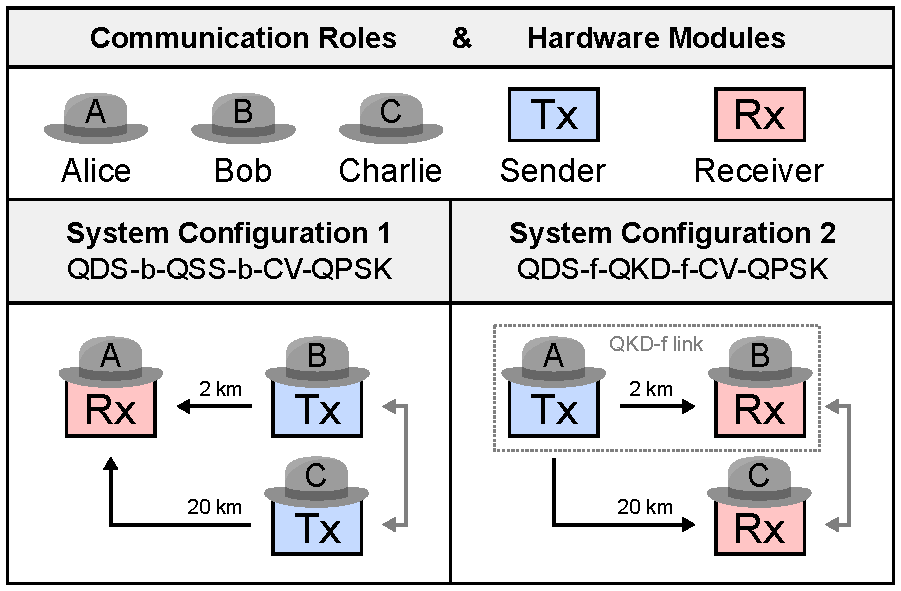
\includegraphics[draft=false, width=0.8\linewidth]{aqc/Fig2_roles-v8}
\caption{\label{fig:agile_tasks} Our two agile quantum systems. Depending on the setup configuration and the chosen task, the hardware modules perform either as Alice or as Bob/Charlie. Tx: hardware sender module. Rx: hardware receiver modules. Hardware specifications are discussed in Sec.~\ref{sec:aqc_experiment}. \emph{Picture credit: Stefan Richter in Ref.~\cite{Richter2020}}}
\end{figure}

We therefore propose two separate agile quantum systems, one which may perform tasks QDS and QSS, and the other which may perform tasks QDS and QKD. We display these two systems in Fig.~\ref{fig:agile_tasks}. The crucial aspect of these two systems is the separation between the abstract user layer defining the roles performed in the protocols, and the hardware layer. For example, the task QDS can be performed in either of the two systems, and Alice can either choose to be the sender of the quantum states or their receiver, depending on available hardware.

We denote our two systems as \systemB \;and \systemF. The labels indicate which of the above cryptographic tasks are supported; the underlying quantum states which they use, and in which direction the quantum states are exchanged ("f" - forward, Alice sends quantum states to Bob and Charlie; or "b" - backward, Bob and Charlie send quantum states to Alice). The forward- or backward- distinction can be seen as analogous to direct- or reverse-reconcilition in QKD \cite{Laudenbach2017}, in which quantum and classical information flow either in the same direction or in opposite directions.

%\MT{Perhaps have a table summarizing each system.}



\clearpage
\section{Agile system \systemB}
%\MT{I'm not sure whether to discuss systemB or systemF first?}
The first agile system we consider runs in the $b$-configuration, Fig.~\ref{fig:agile_tasks}, in which Bob and Charlie are the senders of quantum states while Alice is their receiver. We immediately see that the QSS protocol proposed and analysed in Chapter~\ref{chapter:qss} may be inherited into this agile system, c.f. Fig.~\ref{fig:qss_distribution_stage}. For consistency with notation we will now refer to this QSS protocol as QSS-$b$, and we will analyse it further below in Sec.~\ref{sec:aqc_qssb}.

We also propose a second cryptographic protocol which fits into the system \systemB, which performs the QDS task. We refer to the second protocol as QDS-$b$, and will analyse it below in Sec.~\ref{sec:aqc_qdsb}. Unlike the QDS protocol analysed in Chapter~\ref{chapter:qds}, for QDS-$b$ it is Bob and Charlie who are the senders of quantum states, while Alice is the recipient. %We will describe the protocol below, and then discuss how its security analysis must differ from Chapter~\MT{X}, and demonstrate how it fulfils QDS requirements $1-5$ from Chapter~\MT{X}.
Our first agile system \systemB \; is thus able to perform both QSS and QDS tasks using identical quantum resources. %\MT{Say somewhere my nice line about the quantum stage being "agnostic" to final protocol}

\subsection{Protocol QDS-$b$}

%\MT{I can have a picture about the QDS-b implementation.}

\begin{figure}[htp]
\centering
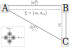
\includegraphics{aqc/qdsb_setup.png}
\caption{\label{fig:qdsb_setup} \MT{TODO: make this figure. I should make the equivalent QDSf one first.}}
\end{figure}

Recall that a QDS scheme must fulfill the requirements from List~\ref{list:qds_requirements} and provide security against a dishonest forger, security against repudiation, and should be robust and succeed when all parties behave honestly, Fig.~\ref{fig:qds_attacks}. We will first outline how protocol QDS-$b$ runs, and then prove that it fulfills each of these requirements.

The protocol QDS-$b$ runs as follows:
%\MT{Make sure it written analogously to QDS-$f$ above.}

\subsubsection*{Distribution stage}

\paragraph{Step $1$.}
For each future message $m \in \left\{0, 1\right\}$ which Alice wishes to securely sign, Bob and Charlie create the classical strings
\begin{equation}
\Phi_m^{\left(B, C\right)} = \left\{\phi_{j, m}^{\left(B, C\right)}\right\}_{j=1}^L
\end{equation}
of length $L$, where the $\phi_j$ are complex phases chosen from the QPSK alphabet. The $\phi_j$ are assumed to be chosen uniformly and at random.
%Bob and Charlie both send Alice a sequence, length $L$, of coherent states chosen randomly from the QPSK alphabet. Bob and Charlie each keep a record of which states they have sent.


\paragraph{Step $2$.} Bob and Charlie form sequences of quantum coherent states corresponding to elements of $\Phi_m^{\left(B, C\right)}$ and distribute them through the quantum channels to Alice. Bob and Charlie each keep a record of $\Phi_m^{\left(B, C\right)}$.

\paragraph{Step $3$.} Alice performs heterodyne detection on each received state and receives complex phase outcomes which we denote $x_{B, C} \in \mathbb{C}$, with the subscript denoting which player send the coherent state. Since measurement is performed immediately on receipt of the state, Alice does not require quantum memory and the remainder of the protocol is entirely classical.

At the end of the quantum stage of the protocol, Alice possesses two classical strings, each of length $L$, which contain her complex phase measurements. She now forms eliminated signatures $A_{B, C}^m$ by writing down which two states from the QPSK alphabet are least-compatible with the $x_{B, C}^j$. The eliminated signatures are formed identically to Fig.~\ref{fig:qds_mismatches}.

\paragraph{Step $4$.} \emph{Symmetrization:} Bob and Charlie swap a random half of their $\Phi_m^{\left(B, C\right)}$ in order to guard against a dishonest Alice. Bob (Charlie) now possesses signature $X_B^m, \left(X_C^m\right)$ which consists of two halves of length $L/2$, one of which was generated by Bob (Charlie), and one of whoch was received during the swapping. Denote the first half by $Y_m^{\left(B\right)}$ and the second half by $Z_m^{\left(B\right)}$ in analogy with Chapter~\ref{chapter:qds}, and similarly for Charlie. Unlike Chapter~\ref{chapter:qds}, strings $Y_m^{\left(B\right)}$ and $Z_m^{\left(B\right)}$ contain phase information, while $A_{B, C}^m$ are eliminated signatures

\subsubsection{Messaging stage}
Messaging may occur any time after distribution.

\paragraph{Step $5$.} Alice sends the classical triplet $\Sigma = \left(m, \sigma_m\right)$ to Bob. The $m$ is the message she would like to convey, and her signature is $\sigma_m = \left(A_B^m, A_C^m\right)$. 

\paragraph{Step $6$.} Bob rearranges $\sigma_m \rightarrow \tilde{\sigma}_m := \left(\tilde{A}_{Y, m}^B, \tilde{A}_{Z, m}^B\right)$ by selecting elements from Alice's declaration which correspond to the two halves of his signature. Bob compares $\tilde{\sigma}_m$ to his two halves and counts the number of mismatches. Message $m$ is accepted as genuine provided that
\begin{equation}
\mathcal{M}\left(Y_m^B, \tilde{A}_{Y, m}^B\right) \le s_B \frac{L}{2} \qq{and} \mathcal{M}\left(Z_m^B, \tilde{A}_{Z, m}^B\right) \le s_B \frac{L}{2}
\end{equation}
otherwise the protocol aborts. %The threshold $s_B$ in general takes a different value from the $s_B$ used in Chapter~\ref{chapter:qds}.

\paragraph{Step $7$.} If Bob has accepted $m$ then he forwards $\Sigma$ to Charlie, who similarly checks for mismatches between Alice's eliminated signature and his signature. Charlie accepts the message if
\begin{equation}
\mathcal{M}\left(Y_m^C, \tilde{A}_{Y, m}^C\right) \le s_C \frac{L}{2} \qq{and} \mathcal{M}\left(Z_m^C, \tilde{A}_{Z, m}^C\right) \le s_C \frac{L}{2}
\end{equation}
otherwise it aborts. %The $s_C$ in general takes a different value from the $s_C$ in Chapter~\ref{chapter:qds}. 
If both Bob and Charlie accept $m$ then the protocol has succeeded. 

It is worth noting some important similarities and differences between QDS-$b$ and the protocol described in Ch.~\ref{chapter:qds}. While both protocols rely on QPSK alphabet, heterodyne detection, and the construction and comparison of eliminated signatures, the security analysis required for the two protocols differs. Crucially, while in Ch.~\ref{chapter:qds} the $j^{\text{th}}$ element of a dishonest forger's declaration is a single phase chosen from QPSK, for QDS-$b$ he must effectively declare \emph{two} phases from QPSK in the form of an eliminated signature element. Additionally, while QDS in Ch.~\ref{chapter:qds} shares similarities with reverse-reconciliation QKD since a forging Bob had to guess Charlie's measurement outcomes, here QDS-$b$ shares similarities with direct-reconciliation QKD as a forging Bob will have to guess Charlie's sent state. We will later see how this affects performance of the protocol. 

\subsection{QDS-$b$ security}
Let us consider the security of QDS-$b$ and check how it fulfils the requirements for a QDS protocol. 

\subsubsection{Security against repudiation}
Recall that during a repudiation attack Alice will try to force Bob and Charlie to disagree about whether her message is genuine. Proof of security against repudiation follows identical lines to Chapter~\ref{chapter:qds}.

We assume that Alice is free to manipulate her declared $A_{B, C}^m$ and she has full control over the mismatch rates $p_B \left(p_C\right)$ with respect to states she originally received from Bob and Charlie. Alice may even choose $p_B$ or $p_C$ to be zero. Security against repudiation arises from the Symmetrizaton step of the protocol. After Bob and Charlie have swapped classical information, they each possess two half-signatures, length $L/2$, consisting either of information which they held originally or which they received during swapping. Alice succeeds in her repudiation attack if Bob accepts both of his halves as genuine while Charlie rejects at least one of his halves as fake. Therefore the probability of successful repudiation is given by

\begin{equation}
\varepsilon_{\text{repudiation}} = \text{P}\left[\left(E_A \cap E_B\right) \cap \left(E_C \cup E_D\right) \right]
\end{equation}

\noindent where the events $E_A, E_B, E_C, E_D$ are defined as

\begin{align}
\mathcal{M}\left(Y_m^B, \tilde{A}_{Y, m}^B\right) \le s_B \frac{L}{2}, \notag \\
%
\mathcal{M}\left(Z_m^B, \tilde{A}_{Z, m}^B\right) \le s_B \frac{L}{2}, \notag \\
%
\mathcal{M}\left(Y_m^C, \tilde{A}_{Y, m}^C\right) > s_C \frac{L}{2}, \qq{and}\notag \\
%
\mathcal{M}\left(Z_m^C, \tilde{A}_{Z, m}^C\right) > s_C \frac{L}{2},
\end{align}
respectively.

Applying probability inequalities Eq.~\ref{eqn:prob_inequality_1},~\ref{eqn:prob_inequality_2} and Hoeffding's inequalities Eq.~\ref{eqn:hoeffding1},~\ref{eqn:hoeffding2}, following the analysis from Sec.~\ref{sec:qds_security_repudiation} we see that

\begin{equation}
\varepsilon_{\text{repudiation}} \le \text{min}\left\{ 2 \; \exp\left(-\left[ p - s_B\right]^2 L\right), 2 \; \exp\left( - \left[ s_C - p\right]^2 L\right) \right\}
\end{equation}
\noindent 
provided that $s_B \le s_C$. The probability $\varepsilon_{\text{repudiation}}$ is maximized when
\begin{equation}
p = \frac{s_B + s_C}{2}.
\end{equation}

\noindent Finally we arrive at,
\begin{equation}\label{eqn:aqc_repudiation}
\varepsilon_{\text{repudiation}} \le 2 \; \exp\left( - \frac{\left[s_C - s_B\right]^2}{4}L\right)
\end{equation}

\noindent identically to Ch.~\ref{chapter:qds}. We have seen that repudiation is only affected by relative mismatch rates between players' signatures and not by who actually possesses the signatures. This is perhaps unsurprising, since in both QDS protocols it is assumed that Alice has complete control over mismatch rates with respect to states held by players before swapping.

\subsection{Robustness}
The robustness of the protocol depends only on parameters $s_B$ and $\perr$. Using Hoeffding inequality Eq.~\ref{eqn:qds_hoeffding2} identically to Sec.~\ref{sec:qds_security_robustness}, we may derive 
\begin{equation}\label{eqn:aqc_robustness}
\varepsilon_{\text{honest abort}} \le 2 \, \exp\left( - \left[s_B - \perr\right]^2 L\right)
\end{equation}
provided that $\perr \le s_B$. The probability $\perr$ of honest mismatch may be modelled as in Sec.~\ref{sec:qds_modelling_perr} and does not change here.

\subsection{Security against forgery}
Since Bob already knows half of Charlie's signature elements (those which Bob himself forwarded) and since $s_B \le s_C$ the most dangerous forger is a dishonest Bob. He is therefore assumed to be the eavesdropper on Charlie's distribution of quantum states, and tries to gain information about the $L/2$ signature elements which Charlie generated himself.

Using Hoeffding's inequalities Eq.~\ref{eqn:qds_hoeffding1} as in Sec.~\ref{sec:qds_security_forgery} we see that at a forging attack succeeds with probability 
\begin{equation}\label{eqn:aqc_forgery}
\varepsilon_{\text{forgery}} \le 2 \; \exp\left( - \left[ \pe - s_C\right]^2 \frac{L}{2} \right)
\end{equation}
provided that $\pe \ge s_C$. 

\subsection{Bounding $\pe$}
All that remains is to bound $\pe$. This will expose several of the differences between QDS-$b$ and QDS from Chapter~\ref{chapter:qds}.

%\MT{I am just copying and pasting the following from Richter2020. Which is fine because I wrote it and it hasn't been edited.}

Consider the $j^\text{th}$ signature element. Charlie holds some $c_j$ denoting which state from the QPSK alphabet he sent. During Messaging, Bob will declare an eliminated signature element, $B_j = \left\{b_j^1, b_j^2\right\}$ which is chosen to minimize $\pe$ and should be the outcome of some optimal strategy on his system, denoted $\mathbb{B}$. The $b_j^1, b_j^2$ correspond to adjacent elements of the QPSK alphabet, with a mismatch occurring if $b_j^1 = c_j$ or $b_j^2 = c_j$. %Additionally, we assume that $B_j$ is the result of some optimal strategy involving Bob's quantum system, $\mathbb{B}_j$.

We define an error variable $\mathcal{E}$ such that 

\begin{equation*}\label{eqn:aqc_error}
\mathcal{E}_j = 
\begin{cases}
1 & \text{if $\mathcal{F}_j$ is eliminated in $\mathcal{G}_j$} \\
0 & \text{otherwise}
\end{cases}
\end{equation*}
which measures whether a mismatch has occurred between $\mathcal{F}_j$ and $\mathcal{G}_j$. Then $\pe \equiv \text{P}\left(\mathcal{E}_j = 1\right)$, and the Shannon entropy $\text{H}\left(\mathcal{E}_j\right) = \text{h}\left(\pe\right)$ is the binary entropy, since $\left|\mathcal{E}_j\right| = 2$. Now, consider the conditional entropy $\text{H}\left(\mathcal{E}_j, b_j^1, b_j^2 \given c_j\right)$. Via the chain rule for conditional entropies,

\begin{equation*}
\text{H}\left(\mathcal{E}_j, b_j^1, b_j^2 \given c_j\right) = \text{H}\left(b_j^1, b_j^2 \given c_j\right)
\end{equation*}

\noindent where we have used the fact that once $b_j^1, b_j^2$ and $c_j$ are known, $\mathcal{E}_j$ is uniquely determined. Using the chain rule on $\text{H}\left(\mathcal{E}_j, b_j^1, b_j^2 \given c_j\right)$ again, but for a different variable, we get

\begin{align*}
\text{H}\left(\mathcal{E}_j, b_j^1, b_j^2 \given c_j\right) &= \text{H}\left(b_j^1, b_j^2 \given \mathcal{E}_j, c_j\right) + \text{H}\left(\mathcal{E}_j \given c_j\right) \notag \\
&\le \text{H}\left(b_j^1, b_j^2 \given \mathcal{E}_j, c_j\right) + \text{h}\left(\pe\right)
\end{align*}

\noindent since conditioning can never increase entropy. Therefore, by expanding the variable $\mathcal{E}_j$,

\begin{align*}
\text{H}\left(b_j^1, b_j^2 \given c_j\right) \le \left(1 - p_e\right) &\text{H}\left(b_j^1, b_j^2 \given \mathcal{E}_j = 0, c_j\right) \\ + &\pe \; \text{H}\left(b_j^1, b_j^2 \given \mathcal{E}_j=1, c_j\right) + \text{h}\left(\pe\right).
\end{align*}

\noindent Now, $\text{H}\left(b_j^1, b_j^2 \given \mathcal{E}_j=0, c_j\right) \le \log_2\left(2\right) = 1$, and similarly for $\mathcal{E}_j=1$, and so

\begin{equation}\label{eqn:A7}
\text{H}\left(b_j^1, b_j^2 \given c_j\right) \le 1 + \text{h}\left(p_e\right).
\end{equation}

\noindent Finally, we expand the conditional entropy in terms of the joint entropy and the mutual information,

\begin{align}\label{eqn:A8}
\text{H}\left(b_j^1, b_j^2 \given c_j\right) &= \text{H}\left(b_j^1, b_j^2\right) - \text{I}\left(b_j^1, b_j^2 : c_j\right) \notag \\
&\ge 2 - \chi\left(b_j^1, b_j^2 : c_j\right)
\end{align}

\noindent where we have used the fact that \emph{a priori} there are four choices for the pair $b_j^1, b_j^2$, and where $\chi$ is the Holevo information. Combining Eqs.~\ref{eqn:A7},~\ref{eqn:A8} we arrive at

\begin{equation}
\text{h}\left(\pe\right) \ge 1 - \chi\left(b_j^1, b_j^2 : c_j\right).
\end{equation}

\noindent Surprisingly this equation has similar form to Eq.~\ref{eqn:qds_hpe}, but with a Holevo information interpreted and calculated differently. %TODO: add a comment about how the Holevo information here is different.


Once $\pe$ and $\perr$ are bounded for the protocol, the probability $\varepsilon_{fail}$ that the protocol fails can be found. For concreteness, we assign equal probability to the failure of the protocol either by allowing a forging or repudiation attack, or by aborting when all players are honest, that is

\begin{equation*}
\varepsilon_{fail} = \varepsilon_{forg} = \varepsilon_{rep} = \varepsilon_{reject}
\end{equation*}

\noindent and by choosing $s_B = p_{err} + \left(p_e + p_{err}\right)/4$; $s_C = p_{err} = 3\left(p_e - p_{err}\right)/4$, in order to satisfy the second two equalities, we arrive at 

\begin{equation}\label{eqn:aqc_qdsb_efail}
\varepsilon_{fail} \le 2 \exp \left[ - \frac{\left( p_e - p_{err} \right)^2}{16} L \right]
\end{equation}

\noindent when $\perr< s_B < s_C < \pe$.

\subsubsection{Calculating Holevo}

Finally, we note that under a beamsplitter attack BS$0$ Bob's \emph{a priori} state is
\begin{equation}
\rho_B = \sum_{k=0}^3 |\sqrt{1-T}\alpha_k\rangle\langle\sqrt{1-T}\alpha_k|
\end{equation}
when states $|\alpha_k\rangle$ from the QPSK alphabet are sent through lossy channel with transmittivity T. Bob's \emph{a posteriori} state is simply $\rho_{B}^k = |\sqrt{1-T}\alpha_k\rangle\langle \sqrt{1-T}\alpha_k|$, from which his Holevo information is calculated as

\begin{equation}
\chi = S\left(\rho_B\right) - \sum_{k=0}^3 p\left(k\right) S\left(\rho_E^k\right)
\end{equation}
with $S$ the Von Neumann entropy. Under attack BS$0$ state $\rho_B^k$ is pure and so $\chi = S\left(\rho_B\right)$. Other attacks may be readily considered, and we present the requisite states in Sec.~\ref{appendix:qdsb_states}. %do this
Bob's mismatch rate $\pe$ may now be calculated and we obtain figure of merit signature length $L$ via Eq.~\ref{eqn:aqc_qdsb_efail}.



\subsection{QDS-$b$ postselection}
Let us apply the postselection technique described in Sec.~\ref{sec:qds_postselection} to protocol QDS-$b$. We shall see that while previously postselection improved efficiency of the protocol, here it is absolutely necessary in order to sign a message for even short distances. We define region $\rps\left(\Delta_r, \Delta_\theta\right)$, Fig.~\ref{fig:rps}, and allow honest recipients to only accept outcomes $x \in \mathbb{C} \setminus \rps$. 

The crucial quantity to consider is $g_{\text{sec}} := \pe - \perr$, measuring the advantage which and honest player has over a dishonest one. The protocol is secure provided that $g_{\text{sec}} > 0$, Eq.~\ref{eqn:aqc_qdsb_efail}. For protocol QDS-$b$, the probability $\pe$ does not depend on Alice's heterodyne measurement, since a dishonest player will attack the sender of the quantum states. Therefore we may reasonably deduce that $\pe$ is unaffected by postselection.

Probability $\perr$ on the other hand is affected by our choice of $\rps$. Given the probability $\text{P}\left(r e^{i \theta} \given \alpha, T\right)$ to obtain complex outcome $r e^{i \theta}$ when state $\ket{\alpha}$ is sent through a noiseless channel with transmission $T$, we see that when no postselection is used
\begin{equation}
\perr = \int\limits_{r=0}^\infty \mathrm{d}r \; r \int\limits_{\theta = \pi/2}^{3\pi/2} \mathrm{d}\theta \; \text{P}\left(r e^{i \theta} \given \alpha, T\right).
\end{equation}

\noindent Incorporating the postselection technique here corresponds to changing the limits of integration, and so when postselection is used we have

\begin{align}
\perr\left(\Delta_r, \Delta_\theta\right) = \frac{1}{\mathcal{N}} \int\limits_{r = \Delta_r}^\infty \mathrm{d}r\; r  &\left[ \int\limits_{\theta = \pi/2 + \Delta_\theta}^{\pi - \Delta_\theta} \mathrm{d}\theta \; \text{P}\left(r e^{i \theta} \given \alpha, T\right)\right. \notag \\
%
&\left. + \int\limits_{\theta = \pi + \Delta_\theta}^{3\pi/2 - \Delta_\theta} \mathrm{d}\theta \text{P}\left(r e^{i \theta}\given \alpha, T\right)\right].
\end{align}





\subsection{QDS-$b$ performance}

\section{Agile system \systemF}
\MT{Let's start talking about the second agile system}

In addition to our first agile system described above, which is capable of switching between QDS and QSS tasks, we here introduce and demonstrate a second agile system, \systemF, which runs in the "f"-configuration Fig.~\ref{fig:agile_tasks} in which Alice is the sender of quantum states, while Bob and Charlie are the states' receivers. As hinted at by this second agile system's name, the system can perform both QDS and QKD tasks. The QKD task in particular already exists in the literature\footnote{Outside of the works which contribute to this Thesis} and so its inclusion demonstrates that pre-existing protocols may be interpreted through an agile lens.

We denote the two protocols as QDS-$f$ and QKD-$f$. QDS-$f$ was studied above in Chapter~\MT{X} and QKD-$f$ was recently analysed in Ref.~\cite{Papanastasiou2018}.

%The QKD task in particular has been the subject of intense study over the past two decades, and the protocol and security proof we utilize for \systemF may already

\subsection{Protocol QDS-$f$}
We leverage the QDS protocol considered in Chapter~\MT{X} to the system \systemF. The protocol, which we here denote QDS-$f$ requires no modification to run over hardware in the $f$-configuration and so the reader is referred to \MT{X} for details and security proof of the protocol. 

In Chapter~\MT{X} a security analysis was performed which assumed ideal behaviour. In Sec.~\MT{X} we relax some of these assumptions and make the protocol analysis more realistic to experimental implementation.

\subsection{Protocol QKD-$f$}
QKD using heterodyne detection of a distributed QPSK alphabet has long been proposed and analysed, owing to its ease of implementation and high compatibility with installed telecommunications infrastructure. \MT{Brief literature review of attempts to analyse security}

A QKD protocol relying on these resources is analysed in Ref.~\cite{Papanastasiou2018}, and it is their analysis which we continue with in this section. 

\MT{Q: how much of this paper should I include?}

%\MT{I should make some graphs and talk about the performance of this protocol. (How close to a lit-review should it be?) <- ahhhh, perfomance will go in the next section}

\section{Performance of CV agile systems}
Let us now consider the theoretical performance of the protocols which contribute to the above agile systems. \MT{Perhaps at some point I should analyse optimal $\alpha$'s for protocols which run on the same system}
\MT{TODO: decide on which graphs to make, and what the story will be here.}

\section{Experimental implementation}
\MT{Briefly describe the experiment and what data I received. I want to make this section stuff which I \emph{didn't} do, so the next section can be stuff which I have actually done.}

An experiment which investigates the above two agile systems was performed at \MT{X} \cite{Richter2020}. Specifically, two optical sender and receiver modules were used to implement the four protocols described above. A sender module (Tx) generates and distributes phase-encoded coherent states chosen from the QPSK alphabet, while a receiver module (Rx) performs heterodyne detection of the received states' phase. Depending on the required configuration, the modules Tx, Rx are variously interpreted as playing roles of Alice or Bob/Charlie, Fig.~\ref{fig:agile_tasks}. 

\begin{figure}[htp]
\centering
\includegraphics{images/aqc_experiment.png}
\caption{\label{fig:aqc_experiment}}
\end{figure}

\subsubsection{Sender module (Tx):} The sender module is depicted in Fig.\ref{fig:aqc_experiment}. An external cavity diode laser (PurePhotonics PPCL-$300$ \MT{cite}) with a linewidth of $15$~kHz is tuned to standard telecom wavelength $1550$~nm and acts as the optical carrier. The carrier beam impinges on a $50:50$ beamsplitter which allows for a shared local oscillator (LO) between modules from one output port. From the other output port  coherent state pulses, chosen randomly from QPSK alphabet $\left\{ \ket{+ \alpha_0}, \ket{i \alpha_0}, \ket{-\alpha_0}, \ket{-i \alpha_0}\right\}$, are prepared by using an I/Q modulator (Fujitsu DP-QPSK $40$~Gbps $LiNbO_3$-integrated)\MT{I'm not sure which word "integrated" should be attached to here}. The I/Q modulator is driven at a rate of $1$~GHz by an arbitrary waveform generator (AWG; Keysight M$8195$A). Finally, a variable optical attenuator (VOA) attenuates the coherent states to a final amplitude of either $\alpha$ or $\alpha^\prime$, with $\alpha \le \alpha^\prime \le \alpha_0$.

The coherent states are then sent through the quantum channel to receiver module Rx.

\subsubsection{Receiver module (Rx):}
Module Rx interferes the received states with the shared local oscillator using the integrated Kylia COH$24$-X $90\si{\degree}$ \MT{what is this?}. The two modules use a shared local oscillator which provides a frame of reference against which heterodyne phase measurement is performed using two balanced optical receivers (Discovery DSC-R$412$) with analog $3$~dB bandwidth of $20$~GHz \MT{what is this?}. In principle the Tx and Rx modules do not need to share a local oscillator and bright phase-reference pulses could be used \MT{cite some stuff.}\footnote{Chat about security loopholes of using shared LO.}

Outputs from the optical receivers are digitized using a digital sampling oscilloscope (Tektronix DPO$77002$SX) with a sampling rate of $25$~GS/s. Finally, proprietary digital signal processing (DSP) algorithms are applied to the quadrature time traces. The DSP consists of a high-pass filter which eliminates low-frequency noise contributions to the signal. Finally, a phase-recovery step is performed using phase-reference states which originally had amplitude $\alpha^\prime$. The signal states carrying quantum information which may now be used for a quantum communications task are those which originally had amplitude $\alpha$.

The Tx and Rx modules were connected by either a $2$~km or $20$~km SMF-$28$ optical fiber link which contributes to a total loss of $0.65$~dB or $4.75$~dB, respectively. This implements the realistic metropolitan distances over which the CV platform is expected to be effective. Experiments were performed for several different signal state modulation amplitudes $\alpha$. For each run of the experiment a total of $1.92\times 10^6$ states were sent in frames of $64$ which consisted of four bright reference pulses ($\alpha^\prime$) followed by $60$ signal pulses ($\alpha$). After the DSP step there remained information on $1.54 \times 10^6$ states. 

\begin{figure}[htp]
\centering
\includegraphics{aqc/experimental_trace.png}
\caption{\label{fig:aqc_experimental_trace} Just Fig.5 from Richter2020}
\end{figure}

An example of some raw output data is displayed in Fig.~\ref{fig:aqc_experimental_trace}. The top of the figure displays raw time trace data, while the bottom displays data after the DSP.

\section{Data analysis}
\MT{Include here what things I need to change for each of the protocols to make them realistic. Include here some analysis of the data.}
\MT{The starting point for this section should be what I received from MPL.}
\MT{What do I want to include here?}


\section{Outlook}

